\chapter{Introduction to routing schemes}
\label{sec:introduction}

Routing is one of the most fundamental problems in the area of distributed
networking. The goal in this problem is to find a distributed algorithm that
allows any source vertex $v$ in a network $G=(V,E)$ to route messages to any
destination vertex $u$, where $u, v\in V$.

Formally, a routing scheme is comprised of two phases. The first phase is
called the preprocessing phase. In this phase $G$ is preprocessed and the
derived routing information is stored locally with the relevant vertices.

In the second phase, the routing phase, the routing scheme allows any vetex to
send messages to any other vertex in a distributed manner.

A naive approach to rountign wo



% \begin{frame}{XY-routing}
%   \begin{figure}
%     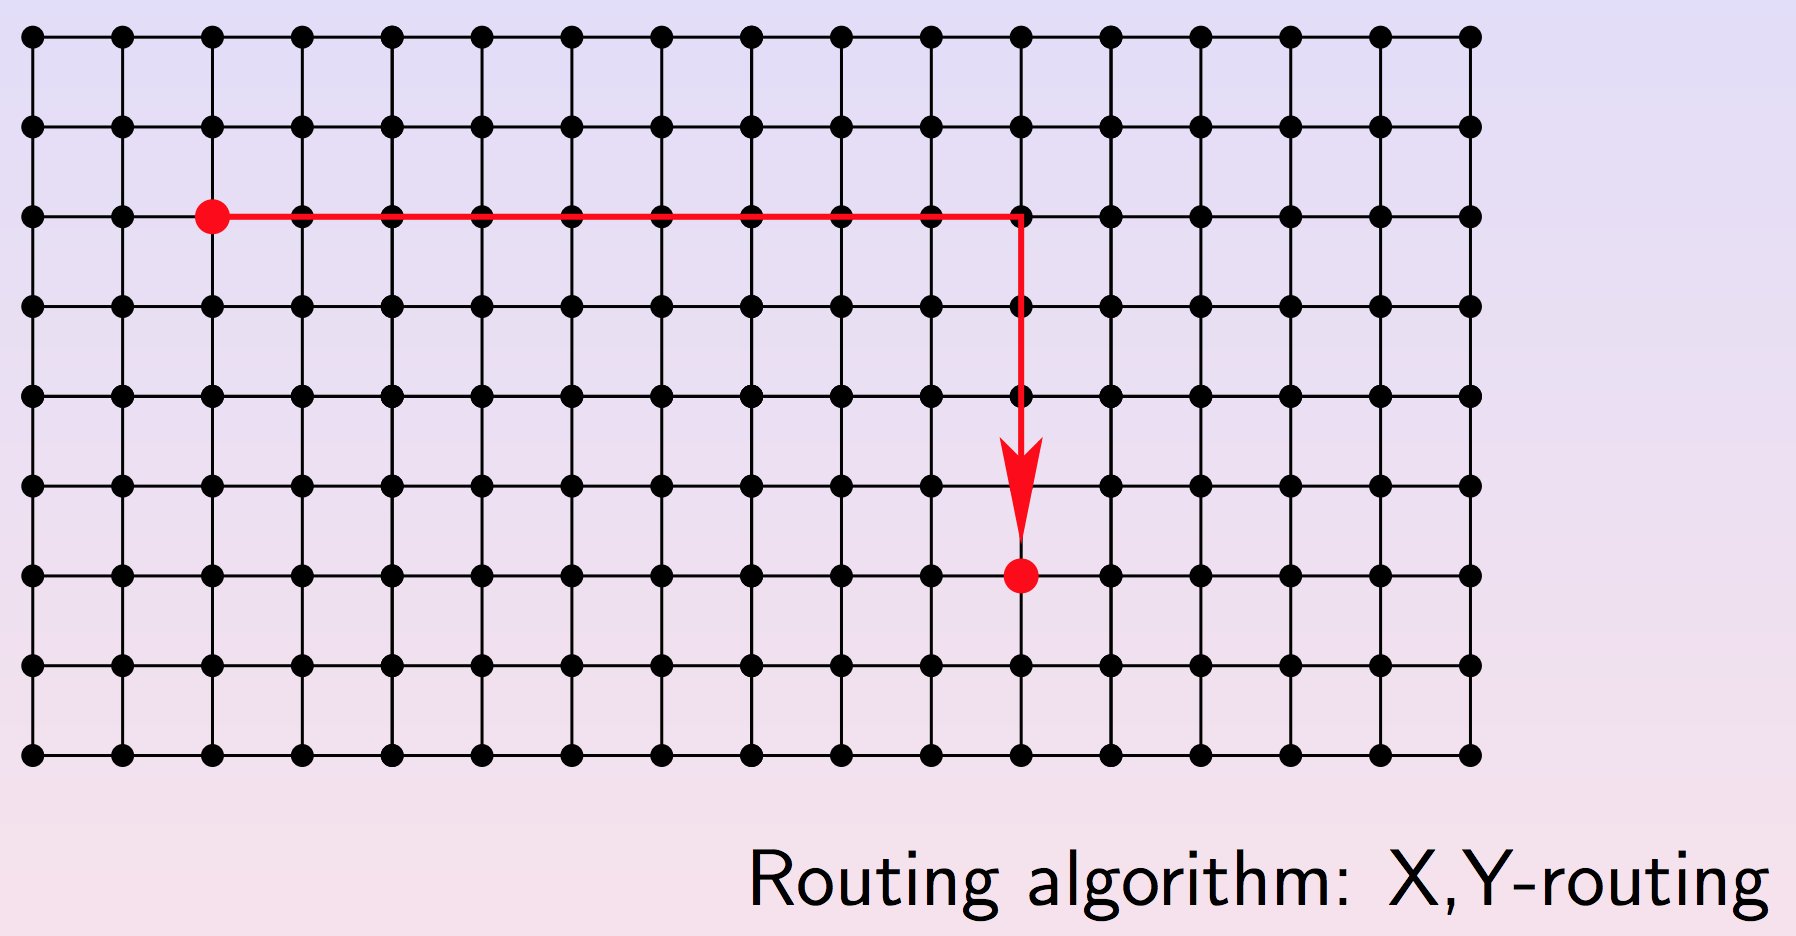
\includegraphics[scale=0.3]{images/xyrouting.png} 
%   \end{figure}
% \end{frame}
% 
% \begin{frame}[fragile]
%   \frametitle{Routing Scheme}
%      
%   \begin{block}{Example: Trivial routing on min cost paths}
%       \begin{itemize}
%         \item On each node, for each of the possible $(n-1)$ destinations,
%         store a port number leading to the next node on a min cost path to the
%         destination.
%         \item Requires each node to store $\Omega (n\; log\; n)$ bits.
%         \item Does not scale very well.
%       \end{itemize}
%   \end{block}
% \end{frame}
% 
% \begin{frame}[fragile]
%   \frametitle{Minimizing parameters}
%   When working with routing, two factors are normally of interest:
%   \begin{description}
%     \item[Stretch] The max ratio over all source-destination pairs between the
%         cost of the path taken by the routing scheme and the cost of a min
%         cost path.
%     \item[Memory] The max number of bits over all nodes stored for the routing
%         scheme. (ballanced is preferred)
%   \end{description}
% \end{frame}
% 
% \begin{frame}[fragile]
%   \frametitle{Labeled Routing or Name-Independent Routing}
% 
%   In labeled routing we can choose a label for each vertex.
%   Lets use coordinates. Now we can easily route. If an aversery
%   label the vertices randomly, routing gets harder.
% 
%   \begin{figure}
%     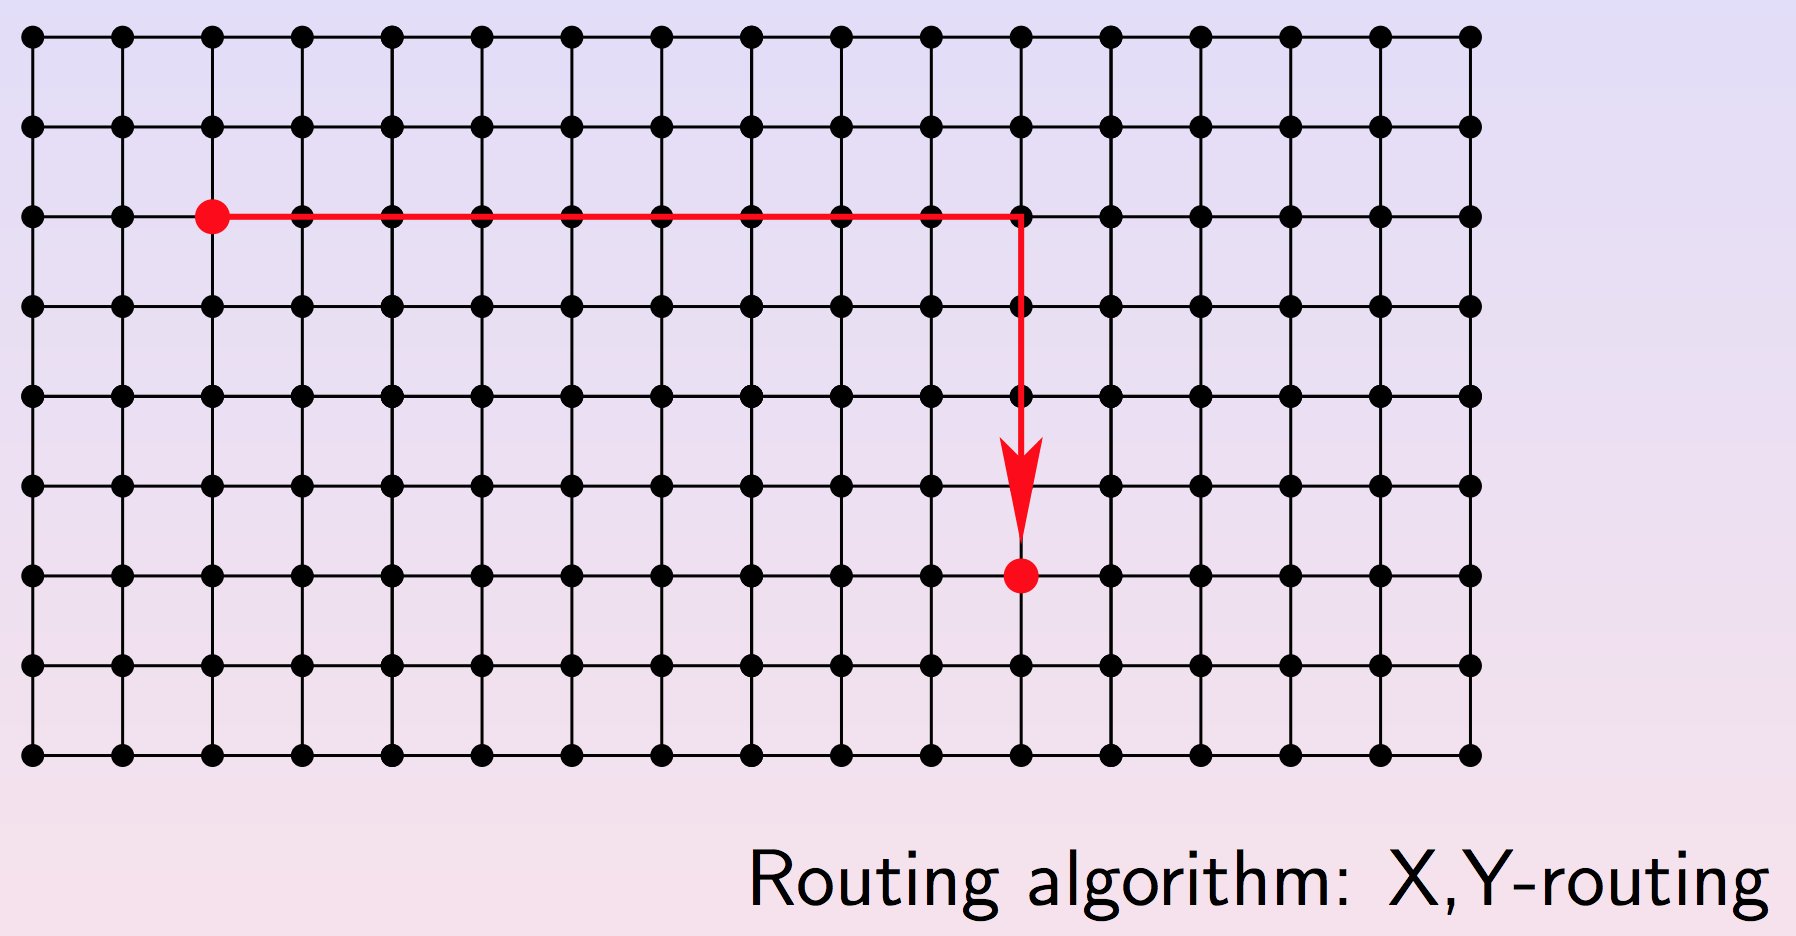
\includegraphics[scale=0.3]{images/xyrouting.png} 
%   \end{figure}
% \end{frame}
% 
% 
% 
% 
% \begin{frame}[fragile]
%   \frametitle{Name-Independent Rounting with min stretch}
%     Given a weighted undirected network with arbitrary node names, we present
%     a compact routing scheme, using a $\tilde{O}(\sqrt{n})$ space routing
%     table at each node and routing along paths of stretch 3.
% 
%     It is known that no compact routing using $o(n)$ space per node can route
%     with stretch below 3. Also, it is known that any stretch below 5 requires
%     $\Omega(\sqrt{n})$ space per node.
% \end{frame}
% 
% \begin{frame}[fragile]
%   \frametitle{Setup}
%     Consider an $n$-node weighted undirected graph $G=(V,E,\omega)$.
% 
%     Each node $v\in V$:
%     \begin{itemize}
%         \item is given a unique name with $O(log\; n)$ bits.
%         \item each outgoing edge is given a unique port name in $\{1,\dots,deg(v)\}$.
%     \end{itemize}
% \end{frame}
